\section{Database}
\subsection{Descrizione}
sqlite3
\subsection{Modello E/R}
\begin{center}
    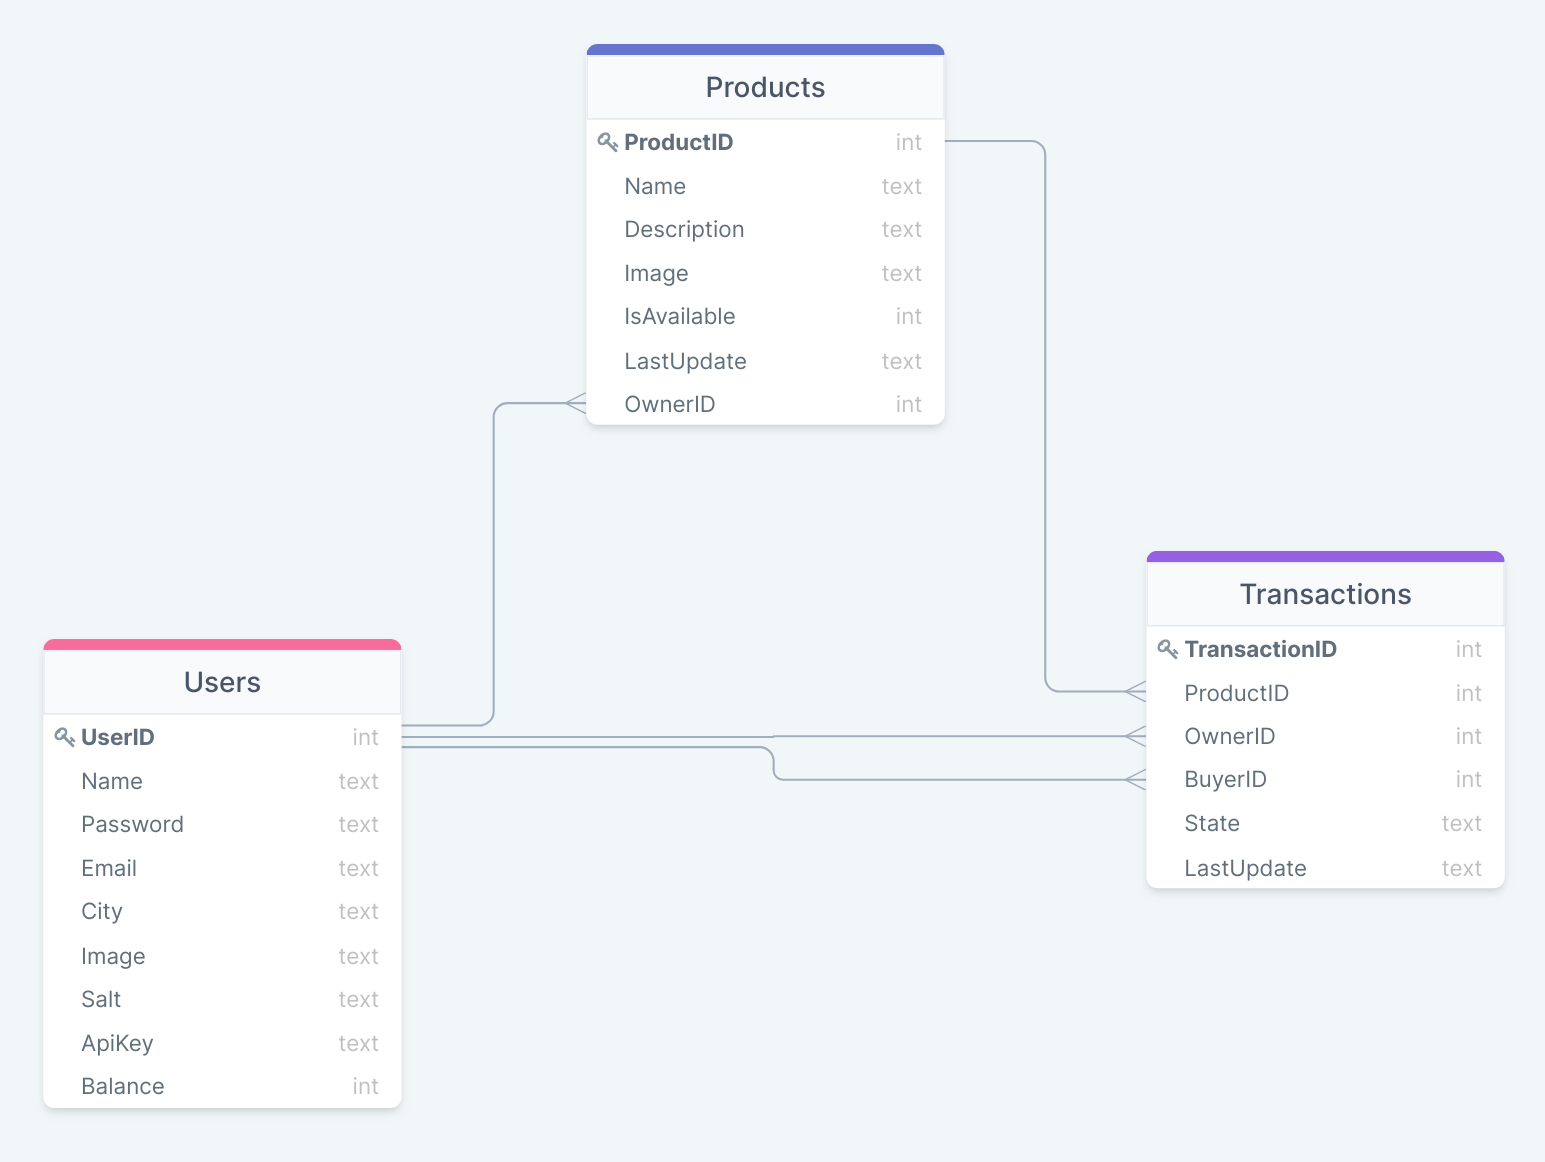
\includegraphics[scale=0.28]{images/modello_e_r.png}
\end{center}
\subsection{Modello logico}
\begin{center}
    \begin{tabular}{ |l|c|l| } 
    \hline
    \multicolumn{3}{|c|}{\textbf{Users}} \\
    \hline
    Nome Campo & Tipo & Note \\
    \hline
    UserID & INTEGER & NOT NULL, PK \\
    Name & TEXT & NOT NULL \\
    Password & TEXT & NOT NULL \\
    Email & TEXT & NOT NULL \\
    City & TEXT & NOT NULL \\
    Image & TEXT & NOT NULL \\
    Salt & TEXT & NOT NULL \\
    ApiKey & TEXT & NOT NULL \\
    Balance & INTEGER & NOT NULL \\
    \hline
    \end{tabular}
\end{center}
\begin{center}
    \begin{tabular}{ |l|c|l| } 
    \hline
    \multicolumn{3}{|c|}{\textbf{Products}} \\
    \hline
    Nome Campo & Tipo & Note \\
    \hline
    ProductID & INTEGER & NOT NULL, PK \\
    Name & TEXT & NOT NULL \\
    Description & TEXT & NOT NULL \\
    Image & TEXT & NOT NULL \\
    IsAvailable & INTEGER & NOT NULL \\
    LastUpdate & TEXT & NOT NULL \\
    OwnerID & INTEGER & NOT NULL, FK(Users) \\
    \hline
    \end{tabular}
\end{center}
\begin{center}
    \begin{tabular}{ |l|c|l| } 
    \hline
    \multicolumn{3}{|c|}{\textbf{Transactions}} \\
    \hline
    Nome Campo & Tipo & Note \\
    \hline
    TransactionID & INTEGER & NOT NULL, PK \\
    ProductID & INTEGER & NOT NULL, FK(Products) \\
    OwnerID & INTEGER & NOT NULL, FK(Users) \\
    BuyerID & INTEGER & NOT NULL, FK(Users) \\
    State & TEXT & NOT NULL \\
    LastUpdate & TEXT & NOT NULL \\
    \hline
    \end{tabular}
\end{center}
\subsection{Entity Framework Core}
db schema generato code-first
code snippets